%
%
% (c) 2020 Michael Schmid, Hochschule Rapperswil
%
% !TEX root = ../presentation.tex

\begin{frame}
  \frametitle{Mathematical Notation}
  \begin{columns}
    \column{0.45\linewidth}
    % $$ \frac {\partial u}{\partial t}+u{\frac {\partial u}{\partial x}}=0 $$
    \begin{itemize}
     \item Discretization
     \begin{itemize}
       \item  $u_i^n$ is the point to be calculated
       \item $i-1$ is a step back in space
       \item $n-1$ is a step back in time
       \item $\Delta t$ is the step size in time
       \item $\Delta x$ is the step size in space

     \end{itemize}
    \end{itemize}
    \column{0.7\linewidth}
    \begin{center}
        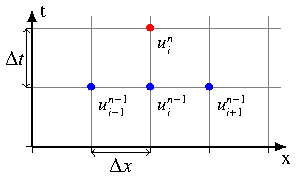
\includegraphics[width=1\textwidth]{../BurgersEquation/tikz/Gitter/gitter.pdf}
      \end{center}
  \end{columns}
  \end{frame}
%
% \begin{frame}
%   \frametitle{Mathematical Notation}
%   $$ \frac {\partial u}{\partial t}+u{\frac {\partial u}{\partial x}}=0 $$
%     $$ \frac {u_{i}^{n-1} - u_{i}^{n}}{\Delta t}+u_{i}^{n}{\frac {\partial u}{\Delta x}}=0 $$
% \end{frame}
